\emph{Vaadin}~\cite{vaadin} es un \textbf{framework} para el desarrollo de aplicaciones \emph{web} avanzadas, también conocidas como \emph{Rich-Internet Applications (RIA)}~\cite{}. El objetivo del paradigma \emph{RIA} es desarrollar aplicaciones \emph{web} con interfaces avanzadas que les haga asemejarse a las aplicaciones de escritorio. La principal ventaja que aporta \emph{Vaadin} es que permite escribir aplicaciones en código Java, como si fuesen de escritorio, y luego este código es transformado para que funcione en tecnologías web como HTML ()~\cite{}, CSS ()~\cite{}, Javascript~\cite{}, HTTP~\cite{} o AJAX ()~\cite{}.

Una de las características diferenciadores de \texttt{Vaadin} es que, al contrario de las librerías de JavaScript tradicionales, \emph{Vaadin} también contempla la parte del servidor, por lo se generan tanto las llamadas al servidor desde la interfaz gráfica (\emph{front-end}) como la recepción y tratamiento de esas llamadas en la parte del servidor (\emph{back-end}). El proyecto LUCA está desarrollado sobre \emph{Vaadin}, por lo que los diferentes elementos desarrollados en este trabajo necesitan comunicarse y correr sobre Vaadin. 

%%========================================================================%%
%% NOTE(Pablo): Rehacerla en castellano o poner de dónde se ha copiado    %%
%%   Prefiero lo primero                                                  %%
%%   ¿Esta figura se referencia desde el texto?                           %%
%%========================================================================%%

\begin{figure}[!tb]
    \centering
	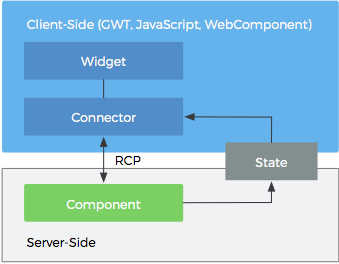
\includegraphics[scale=1.5]{schema.png}
	\caption{Arquitectura Básica de Vaadin}
\label{fig:schema}
\end{figure}

El primer paso para comprender el funcionamiento de \emph{Vaadin} es entender su arquitectura básica (Figura~\ref{fig:vaadinInteraction)} representa brevemente esta interacción. Como podemos observar, se consta de tres módulos bien diferenciados. El primer módulo se corresponde con el proyecto implementado en Java. El segundo con el conector en javascript que servirá de comunicador o intermediario entre la librería Javascript y el proyecto. El último se corresponde con la librería Javascript, un ejemplo de esta es GoJS, explicada previamente, por lo tanto, no se mencionará más de ella más allá de que es la encargada del entorno gráfico.

 			
 	
 	\begin{figure}[!tb]
 		\centering
 		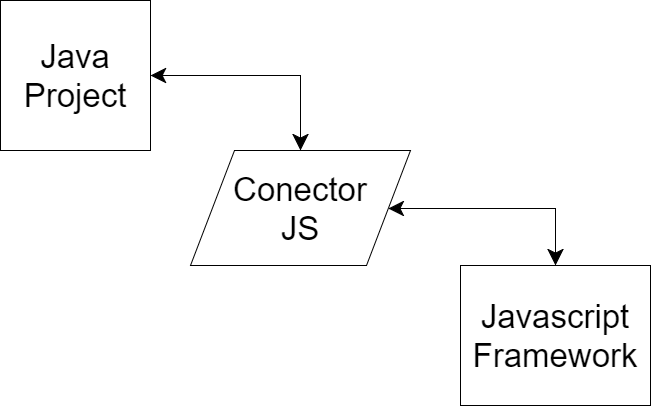
\includegraphics[scale=0.5]{vaadinInteraction.png}
 		\caption{Interacción Vaadin}\label{fig:vaadinInteraction}
 	\end{figure}
 	
 	
 	
 			
 En este proyecto la pieza central que será la encargada de comunicarse con el conector será un componente abstracto que implementa \emph{Vaadin} para llevar a cabo esta finalidad.

Este componente consta de dos partes, por un lado tiene una clase que extiende de \emph{AbstractJavaScriptComponent} (Figura~\ref{fig:componenteVaadin}~,~Línea 2) que será la pieza que posea el contexto para comunicarse con el conector, además, en esta parte se especificarán todos los ficheros javascript u hojas de estilo que sean necesarios (Figura~\ref{fig:componenteVaadin}~,~Línea 1). Por otro lado el estado de dicho componente, que se encargará de asegurar la integridad de los elementos que existen dentro del componente y extenderá de \emph{JavaScriptComponentState} (Figura~\ref{fig:estadoComponenteVaadin}~,~Línea 1).
 	
 	\begin{figure}[!tb]
 		\centering
 		\begin{lstlisting}[language=Java]
	 	@JavaScript({ "connector.js" })
	 	public class Component extends AbstractJavaScriptComponent {
		 	public Component(String content) {
		 		getState().content = content;
		 	}
		 	
		 	@Override
		 	protected ComponentState getState() {
		 		return (ComponentState) super.getState();
		 	}
	 	}
 		\end{lstlisting}
 		\caption{Componente Vaadin}
 		\label{fig:componenteVaadin}
 	\end{figure}


 \begin{figure}[!tb]
 	\centering
 	\begin{lstlisting}[language=Java]
	public class ComponentState extends JavaScriptComponentState {
		public String content;
	}
 	\end{lstlisting}
 	\caption{Estado Componente Vaadin}
 	\label{fig:estadoComponenteVaadin}
 \end{figure}


	La comunicación del componente con el conector se puede realizar de varias formas, las más comunes son:
	\begin{itemize}
		\item  Cambiando el estado del componente, ya que se ejecutará automáticamente una llamada en el conector por dicho cambio.
		\item  Haciendo una llamada al conector mediante una función previamente publicada (Figura~\ref{fig:callfunction}~,~Línea 1). De esta forma se puede elegir la función a la que llamar pasando una serie de parámetros.
	\end{itemize}

\begin{figure}[!tb]
	\centering
	\begin{lstlisting}[language=JavaScript]
	callFunction("updateState",content);
	\end{lstlisting}
	\caption{Llamada al conector}
	\label{fig:callfunction}
\end{figure}
 			
 			
 			
 	\subsubsection{Javascript Connector}	
 	
 	
 	El conector es el encargado de comunicarse con ambos lados, es decir, con el proyecto Java y el framework Javascript.
 	
 	Se empieza con la declaración de la localización del conector bajo la nomenclatura \emph{window+dirección+nombre del conector}, y después se especifica el conector (Figura~\ref{fig:conectorDesc}~,~Línea 1).
 	
 	El conector se compone principalmente de una función que se ejecuta cuando el estado del Componente en Vaadin cambia (Figura~\ref{fig:conectorDesc}~,~Líneas~04-06). Además, se le pueden añadir todas las funciones necesarias para el correcto funcionamiento (Figura~\ref{fig:conectorDesc}~,~Líneas~08-10). Como se puede observar en la Figura~\ref{fig:conectorDesc}~,~Línea~03, se crea un componente, este componente se correspondería, aplicando el caso al que se utilizará posteriormente en el proyecto, a GoJS, más concretamente a la descripción que se explica en el ejemplo del mismo.
 	
 	
 	\begin{figure}[!tb]
 		\centering
 		\begin{lstlisting}[language=JavaScript]
 		window.urlPaquete_connector = function() {

 			var mycomponent = new mylibrary.MyComponent(this.getElement());
		 	
		 	this.onStateChange = function() {
		 		mycomponent.content = this.getState().content;
		 	}
		 	
		 	this.updateState = function(content){
		 		mycomponent.content = content;
		 	}
	 	}
 		\end{lstlisting}
 		\caption{Conector}
 		\label{fig:conectorDesc}
 	\end{figure}

	En conclusión, se ha explicado un ejemplo de interacción del componente Vaadin con un Framework Javascript a través de un conector Javascript.
 	
 	
 	
 			